% vim: set textwidth=78 autoindent:

%\subsection{Decorations Plugins}
\subsection{Extensions Décorations}

% when the revision of a section has been finalized, 
% comment out the following line:
% \updatedisclaimer

%The Decorations Plugins includes the Copyright Label Plugin, the North 
%Arrow Plugin and the Scale Bar Plugin. They are used to ``decorate'' the 
%map by adding cartographic elements.
Les extensions Décorations incluent les extensions Etiquette Copyright,
Flèche Nord et Echelle Graphique. Elles sont destinées à "habiller" la carte
en ajoutant des éléments cartographiques.

%\subsubsection{Copyright Label Plugin}
\subsubsection{l'extension Etiquette Copyright}

%The title of this plugin is a bit misleading - you can add any random text to the map.
Le nom de cette extension est sujet à confusion : elle permet d'ajouter n'importe quelle étiquette de texte à la carte.

%\begin{figure}[ht]
%   \begin{center}
%   \caption{Copyright Label Plugin \nixcaption}\label{fig:copyright}\smallskip
%   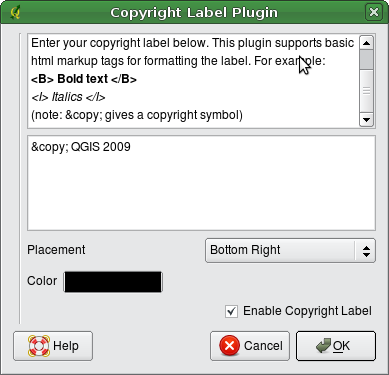
\includegraphics[clip=true, width=8cm]{copyright}
%\end{center}  
%\end{figure}
\begin{figure}[ht]
   \begin{center}
   \caption{l'extension Etiquette Copyright\nixcaption}\label{fig:copyright}\smallskip
   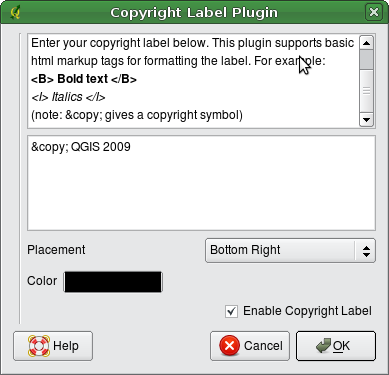
\includegraphics[clip=true, width=8cm]{copyright}
\end{center}
\end{figure}

%\begin{enumerate}
%\item Make sure the plugin is loaded
%\item Click on \mainmenuopt{Plugins} > \dropmenuopt{Decorations} > \dropmenuopttwo{copyright_label}{Copyright Label} or use the \toolbtntwo{copyright_label}{Copyright Label} %button from the Toolbar.
%\item Enter the text you want to place on the map. You can use HTML as
%  shown in the example
%\item Choose the placement of the label from the \selectstring{Placement}{Bottom Right} drop-down box
%\item Make sure the \checkbox{Enable Copyright Label} checkbox is checked
%\item Click \button{OK} 
%\end{enumerate}
\begin{enumerate}
\item Assurez-vous que l'extension soit chargée.
\item Cliquez sur \mainmenuopt{Plugins} > \dropmenuopt{Décorations} > \dropmenuopttwo{copyright_label}{Etiquette de Copyright} ou utilisez le bouton \toolbtntwo{copyright_label}{Etiquette de Copyright} dans la barre d'outils.
\item Entrez le texte que vous souhaitez placer sur la carte. Vous pouvez utiliser le HTML, comme
  indiqué dans l'exemple.
\item Choisissez la position de l'étiquette depuis la liste de choix déroulant \selectstring{Placement}{Coin Inférieur Droit}.
\item Assurez-vous que la case \checkbox{Activer l'étiquette du copyright} soit cochée.
\item Cliquez sur \button{OK}.
\end{enumerate}

%In the example above, the first line is in bold, the second (created using
%\textless br\textgreater) contains a copyright symbol, followed by our company name in
%italics.
Dans l'exemple ci-dessus, la première ligne est en gras, la seconde (créée avec
\textless br\textgreater) contient un symbole copyright, suivi par le nom de notre société
en italique.

%\subsubsection{North Arrow Plugin}
\subsubsection{L'extension Flèche Nord}

%The North Arrow plugin places a simple north arrow on the map canvas. At
%present there is only one style available. You can adjust the angle of the
%arrow or let QGIS set the direction automatically. If you choose to let
%QGIS determine the direction, it makes its best guess as to how the arrow
%should be oriented. For placement of the arrow you have four options, 
%corresponding to the four corners of the map canvas.
L'extension Flèche Nord place une simple rose des vents sur la carte. Un seul
style est disponible pour le moment. Vous pouvez ajuster l'angle de la flèche 
ou laisser QGIS déterminer automatiquement la direction. Si vous faites ce 
dernier choix, QGIS essaiera de calculer la meilleure orientation de la flèche.
Quatre options sont disponibles pour la position de la flèche, qui correspondent
au quatre coins de la fenêtre carte.

%\begin{figure}[ht]
%   \begin{center}
%   \caption{North Arrow Plugin \nixcaption}\label{fig:north_arrow}\smallskip
%   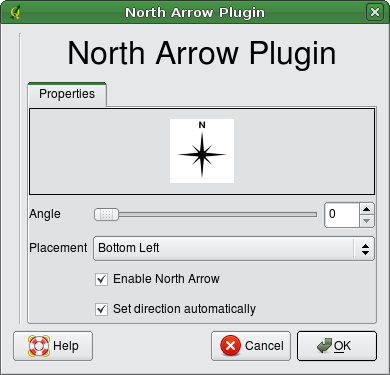
\includegraphics[clip=true, width=8cm]{north_arrow_dialog}
%\end{center}  
%\end{figure}
\begin{figure}[ht]
   \begin{center}
   \caption{L'extension Flèche Nord \nixcaption}\label{fig:north_arrow}\smallskip
   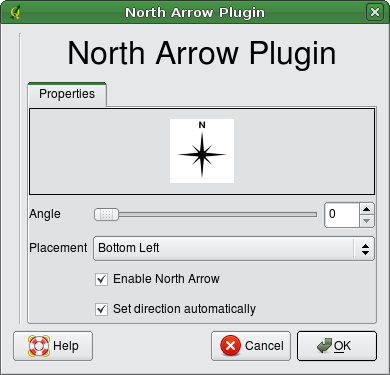
\includegraphics[clip=true, width=8cm]{north_arrow_dialog}
\end{center}  
\end{figure}

%\subsubsection{Scale Bar Plugin}
%The Scale Bar plugin adds a simple scale bar to the map canvas. You
%control the style and placement, as well as the labeling of the bar.
\subsubsection{L'extension Échelle Graphique}
L'extension Échelle Graphique ajoute une simple échelle graphique à la carte.
Vous pouvez contrôler le style et la position, ainsi que l'étiquetage de l'échelle.

%QGIS only supports displaying the scale in the same units as your map frame. So
%if the units of your layers are in meters, you can't create a scale bar in
%feet. Likewise if you are using decimal degrees, you can't create a scale
%bar to display distance in meters.
L'échelle ne peut afficher que les mêmes unités que celles de votre fenêtre carte.
Si les unités des couches sont en mètres, vous ne pourrez pas créer une échelle en
pieds. De la même manière, si vous utilisez les degrés décimaux, vous ne pourrez 
pas créer une échelle en mètres.

%To add a scale bar:
Pour ajouter une échelle graphique :

%\begin{enumerate}
%\item Click on \mainmenuopt{Plugins} > \dropmenuopt{Decorations} > \dropmenuopttwo{scale_bar}{Scale Bar} or use the \toolbtntwo{scale_bar}{Scale Bar} button from the Toolbar.
%\item Choose the placement from the \selectstring{Placement}{Bottom Left} drop-down list
%\item Choose the style from the \selectstring{Scale bar style}{Tick Down} list
%\item Select the color for the bar \selectcolor{Color of bar}{black} or use the default black color
%\item Set the size of the bar and its label \selectnumber{Size of bar}{30 degrees}
%\item Make sure the \checkbox{Enable scale bar} checkbox is checked
%\item Optionally choose to automatically snap to a round number when the
%  canvas is resized \checkbox{Automatically snap to round number on resize}
%\item Click \button{OK} 
%\end{enumerate}
\begin{enumerate}
\item Cliquez sur \mainmenuopt{Plugins} > \dropmenuopt{Decorations} > \dropmenuopttwo{scale_bar}{Echelle graphique} ou sur le bouton \toolbtntwo{scale_bar}{Echelle graphique}  de la barre d'outils.
\item Choisissez la position depuis la liste de choix déroulant \selectstring{Placement}{Coin Inférieur Gauche}.
\item Choisissez le style depuis la liste de choix déroulant \selectstring{Scale bar style}{Marquage Inférieur}.
\item Choisissez la couleur de l'échelle \selectcolor{Color of bar}{black} ou utilisez le noir par défaut.
\item Choisissez la taille et l'étiquette de l'échelle \selectnumber{Size of bar}{30 degrés}.
\item Assurez-vous que la case \checkbox{Activer l'échelle graphique} soit cochée.
\item Vous pouvez choisir optionnellement d'arrondir automatiquement -l'échelle
 à chaque changement de niveau de zoom \checkbox{Arrondir automatiquement lors du changement de zoom}
\item Cliquez sur \button{OK}.
\end{enumerate}

%\begin{figure}[ht]
%   \begin{center}
%   \caption{Scale Bar Plugin \nixcaption}\label{fig:scale_bar}\smallskip
%   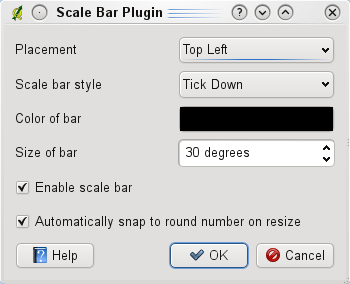
\includegraphics[clip=true, width=8cm]{scale_bar_dialog}
%\end{center}  
%\end{figure}
\begin{figure}[ht]
   \begin{center}
   \caption{L'extension échelle graphique \nixcaption}\label{fig:scale_bar}\smallskip
   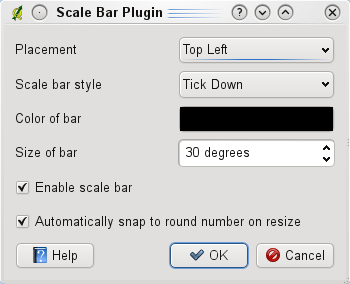
\includegraphics[clip=true, width=8cm]{scale_bar_dialog}
\end{center}  
\end{figure}
